\documentclass{standalone}
\usepackage{pgfplots}
\pgfplotsset{compat=newest}

\begin{document}
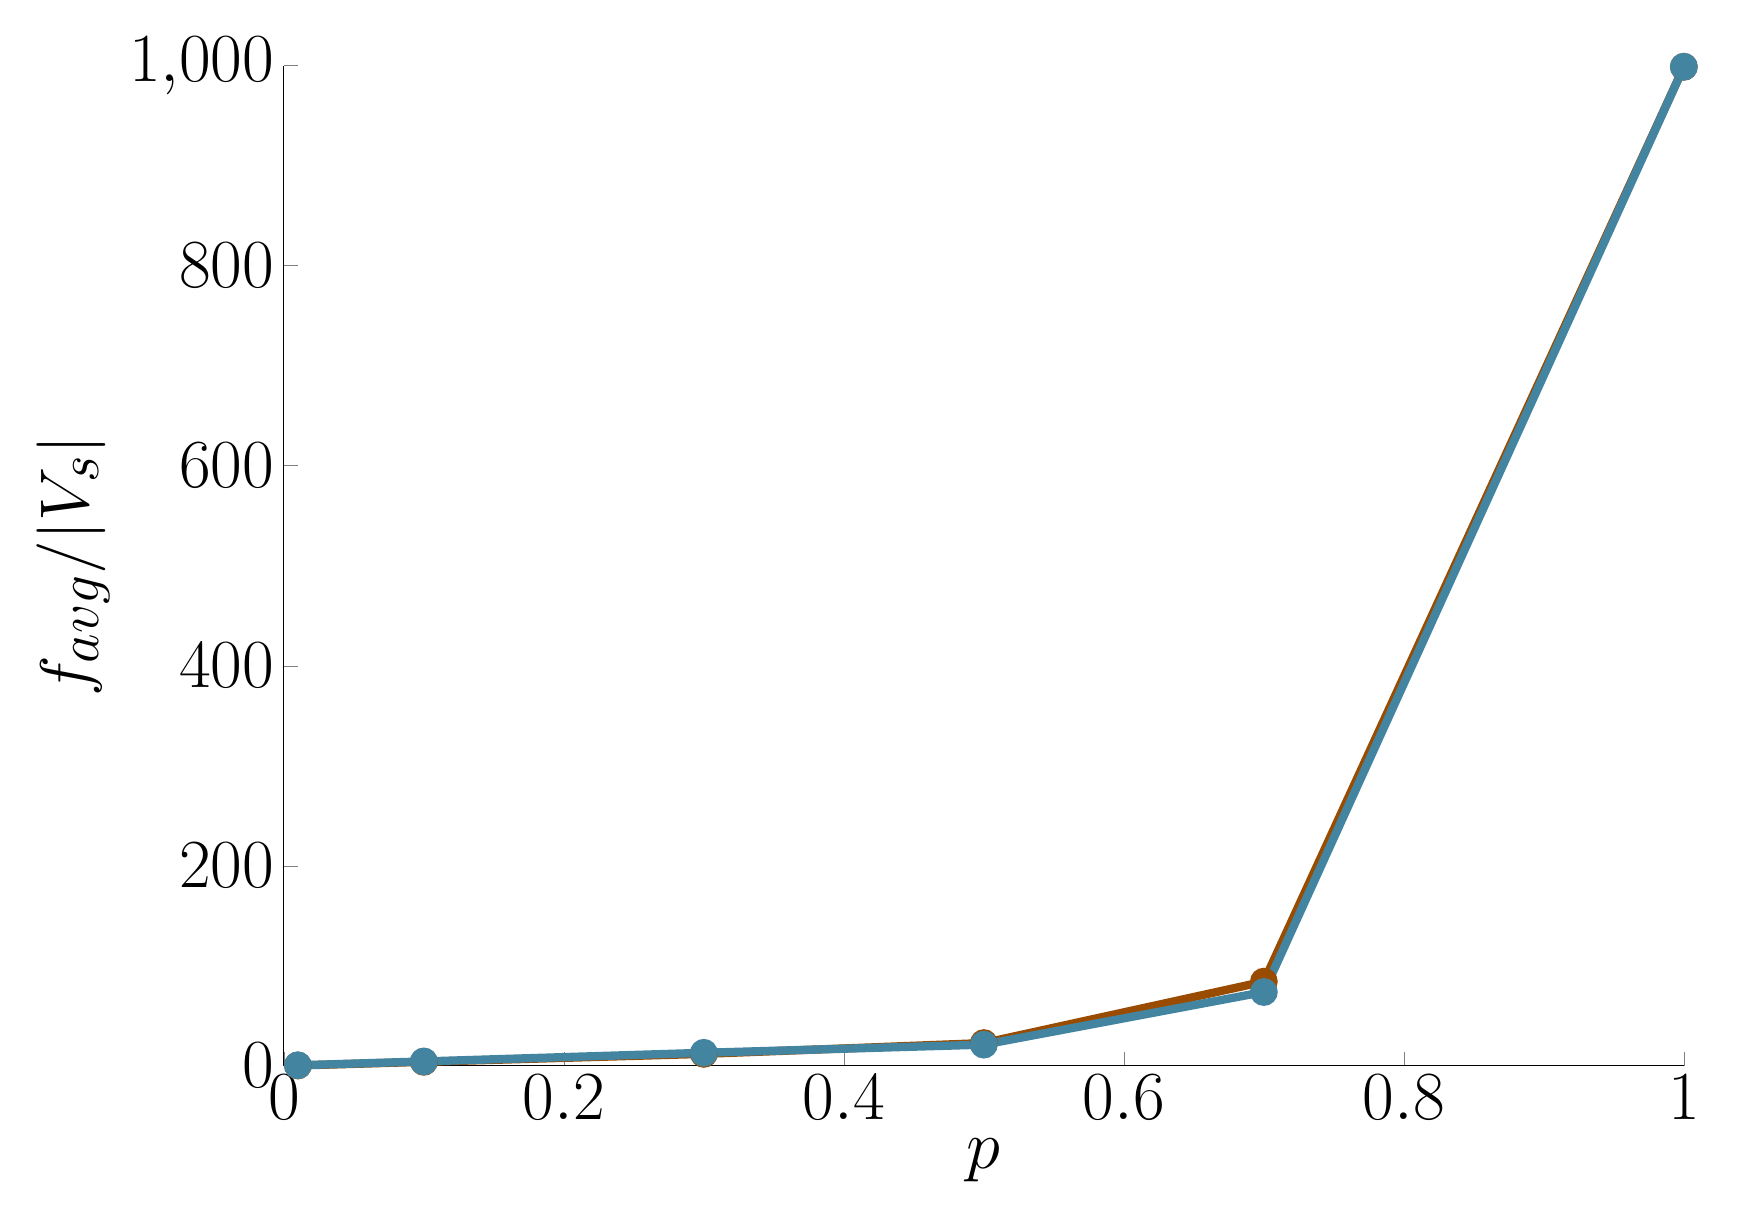
\begin{tikzpicture}

\begin{axis}[%
tick label style={font=\Huge},
label style={font=\Huge},
legend style={font=\Huge},
view={0}{90},
width=7in,
height=5in,
scale only axis,
xmin=0, xmax=1,
xtick={0, 0.2, 0.4, 0.6, 0.8, 1},
xlabel={$p$},
ymin=0, ymax=1000,
ytick={0, 200, 400, 600, 800, 1000},
ylabel={$f_{avg} / |V_s|$},
major tick length=5pt,
axis lines*=left,
legend cell align=left,
clip=false]

\addplot [
mark=*,
mark size=3.5pt,
color=orange!60!black,
solid,
line width=3pt
]
coordinates{
(0.01,0.288)(0.1,3.939)(0.3,11.909)(0.5,22.7236111111)(0.7,84.1545454545)(1,999.0)
};

\addplot [
mark=*,
mark size=3.5pt,
color=cyan!60!black,
solid,
line width=3pt
]
coordinates{
(0.01,0.499912887165)(0.1,4.353)(0.3,12.992)(0.5,21.1294835745)(0.7,73.7637657889)(1,999.0)
};

\end{axis}
\end{tikzpicture}
\end{document}
